El sistema ferroviario de un país cubre un gran conjunto de su territorio. El mismo permite realizar diferentes viajes con transbordos entre distintos ramales y subramales que pasan por sus principales ciudades. Dentro de su proceso de mejoramiento del servicio buscan que ante una emergencia en una estación se pueda llegar de forma veloz y eficiente. Consideran que eso se lograría si el equipo de socorro se encuentra en esa misma estación o en el peor de los casos en una estación vecina (que tenga una trayecto directo que no requiere pasar por otras estaciones). Como los recursos son escasos desean establecer la menor cantidad de equipos posibles (un máximo de k equipos pueden solventar). Se solicita nuestra colaboración para dar con una respuesta a este problema. \\

Se pide:

1. Utilizar el problema conocido como “set dominante” para demostrar que corresponde a un problema NP-Completo.

2. Asimismo demostrar que el problema set dominante corresponde a un problema NP-Completo.

3. Con lo que demostró responda: ¿Es posible resolver de forma eficiente (de forma “tratable”) el problema planteado? \\

HINT: podría ser una buena idea utilizar 3SAT o VERTEX COVER. \\

\section{}

En este problema podemos considerar las ciudades como vertices de un grafo y las aristas como los caminos que los conectan. \\
El problema presentado se puede resolver como el problema del set dominante, en este problema se busca un subset de vertices 'T' tal que todos los vertices que no estan en T sean adyacentes a al menos a un vertice que pertenezca a este subset.\\
Lo que debemos hacer es encontrar el numero minimo de vertices con los que podemos formar T, puesto que este problema se trata de elegir la cantidad minima de equipos de supervivencia para cubrir todas las ciudades y sus adyacentes, con lo que estariamos cumpliendo con el requerimiento pedido\\ 

 \begin{center}
    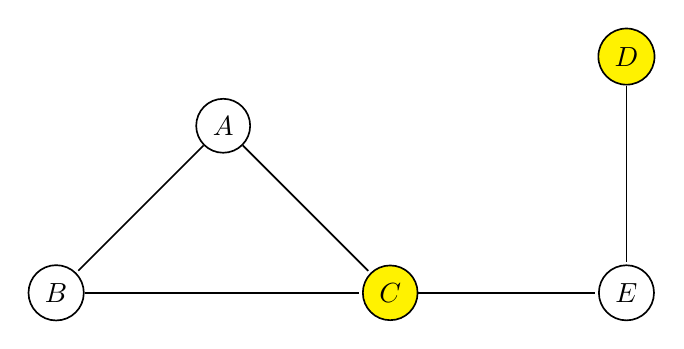
\begin{tikzpicture}[
            thick, 
            main/.style = {draw, circle}, 
            > = stealth, % arrow head style
            shorten > = 1pt, % don't touch arrow head to node
            auto,
            node distance = 3cm, % distance between nodes
            semithick % line style
        ]
        \node[main] (a) {$A$};
        \node[main] (b) [below left of=a] {$B$};
        \node[main] (c) [below right of=a, fill=yellow] {$C$}; 
        \node[main] (e) [right of=c] {$E$};
        \node[main] (d) [above of=e, fill=yellow] {$D$};

        \path[-] (a) edge node {} (b);
        \path[-] (a) edge node {} (c);
        \path[-] (b) edge node {} (c);
        \path[-] (c) edge node {} (e);
        \path[-] (d) edge node {} (e);
    \end{tikzpicture} 
\end{center}

En este caso vemos como las ciudades coloreadas son las que deberian tener el equipo de socorro, puesto que se cubren a si mismas y a las adyacentes, llegando asi a todas las ciudades\\ 
Con esto explicado sabemos que si el problema del set dominante es NP-completo por consiguiente nuestro problema tambien lo sera

\section{}


    Para demostrar que un problema es NP-Completo basta con elegir un problema $Y \in NP-Completo$ y reducirlo polinomialmente a nuestro problema. Para ello podemos elegir el problema de vertex cover que es parte de los problemas NP Completos.\\
    
    Cada instancia del problema de vertex cover consiste de un grafo $G = (V,E)$ y un numero k que sera el numero con el que intentaremos crear un subset de vértices que cubra todo el grafo. Para reducir este problema a uno de set dominante podemos modificar el grafo que tenemos de forma tal que el set dominante nos devuelva si se puede resolver el problema con el mismo numero k para el set dominante y para el vertex cover. La forma de crear el grafo seria para cada arista E que una a los vértices {u,v} del grafo G, crear un nuevo vértice auxiliar {uv} y unirlo a estos dos vértices {u} y {v} formando así triángulos \\

    El nuevo grafo G' puede crearse en tiempo polinomial agregando las aristas correspondientes a los nuevos vértices en tiempo O(V+E).
    La prueba de que esto funciona viene dado por las siguientes afirmaciones: \\
    
    Si algún problema es un NP, entonces, dado un 'certificado', que es una solución al problema y una instancia del problema (en este caso, un grafo $G$ y un entero positivo $k$), se podrá verificar, comprobando si la solución dada es correcta o no, el certificado en tiempo polinomial.\\

El certificado es una secuencia de vértices que forman un Set Dominante en el grafo. Podemos validar esta solución comprobando que:\\
i. todos los vértices pertenecen a los vértices del grafo,\\
ii. todos los vértices que no forman parte de esta secuencia son adyacentes a algunos de los vértices de este conjunto.\\

Esto se puede hacer en tiempo polinomial, es decir $O(V + E)$ usando la siguiente estrategia:\\

flag = verdadero

para cada vertice v en V:

\>\>\>\>\>     si v no pertenece al Set Dominante:

\>\>\>\>\>     \>\>\>\>\>     verificar el conjunto de aristas correspondientes a v

\>\>\>\>\>     \>\>\>\>\>     si v no es adyacente:

\>\>\>\>\>     \>\>\>\>\>     \>\>\>\>\>     para cada uno de los vertices en el Set Dominante: 

\>\>\>\>\>     \>\>\>\>\>     \>\>\>\>\>     \>\>\>\>\>     flag = falso
           
si (flag)

\>\>\>\>\>     la solucion es correcta

sino

\>\>\>\>\>     la solucion es incorrecta\\


Ahora, sin embargo, para probar que un Set Dominante es un NP-Hard, habrá que reducir algún problema NP-Hard que conozcamos a este problema. Haremos una reducción desde el problema de Cobertura de Vértices al del problema del Set Dominante.\\

Cada paso del problema de Cobertura de Vértices consta de un grafo $G$, con $V$ vértices y $E$ aristas, y un entero $K$ que consta del subconjunto de vértices, ya que la entrada se puede convertir en un nuevo problema del Set Dominante. Este nuevo problema tendrá un grafo $G'$, con $V'$ vértices y $E'$ aristas= ($V'$, $E'$).\\

Este nuevo grafo $G'$ será construido de la siguiente manera:\\

\textbf{$E’$}:

\>\>\>\>\>     Para cada arista del grafo $G$, cuyos vértices que conecta son $a$ y $b$:

\>\>\>\>\>     \>\>\>\>\>     Agregar un nuevo vértice $v$

\>\>\>\>\>     \>\>\>\>\>     Unirlo con $a$

\>\>\>\>\>     \>\>\>\>\>     Unirlo con $b$\\

Se genera, entonces, por cada arista del grafo $G$, un nuevo vértice $v$ con dos aristas.\\

\textbf{$V’$}: Agregar todos los vértices $V$ del grafo original $G$.\\

Este nuevo grafo $G’$ se puede obtener en tiempo polinomial: el agregar nuevas aristas por cada nuevo vértice conlleva una complejidad temporal $O(V + E)$. Esta reducción puede probarse mediante las siguientes dos afirmaciones:\\

\begin{itemize}

\item Supongamos que el grafo $G$ tiene una cubierta de vértices $CV$ de tamaño $k$. Cada arista en $G$ tiene uno de los vértices que pertenecen a CV. Por lo tanto, para cada arista e, que consta de vértices \{$a$, $b$\}, al menos $a$ o $b$ es parte de CV. Entonces, si $a$ está contenido en $CV$, por ende el vértice adyacente es $b$, también está cubierto por alguno de los elementos en $CV$. Es decir,\\

$a$,$b$ vértices unidos por $e$ arista

$a$ $\in$ CV \>\>\>\>\>      $\vee$ \>\>\>\>\>      $b$ $\in$  CV

$b$ adyacente a $a$ \>\>\>\>\>     $\Rightarrow$ \>\>\>\>\>     $b$ cubierto por $w$ $\in$ CV\\       	 

Ahora, para todos los vértices $ab$ recientemente agregados por cada arista, el vértice es adyacente tanto a $a$ como a $b$, uno de los cuales es al menos parte de CV, como se demostró anteriormente. Por lo tanto, los vértices adicionales para todas las aristas también están cubiertos por $CV$.\\

Además, el conjunto de vértices que forman la cobertura de vértices de tamaño $k$ conforman el set dominante en el grafo $G’$. Por lo tanto, si $G$ tiene una cobertura de vértices, $G’$ tiene un set dominante del mismo tamaño. Es decir, 

\begin{center}tamaño CV($G$) = tamaño SD($G'$)\end{center}


\item Suponemos que el grafo $G’$ tiene un set dominante de tamaño $k$. Pueden surgir dos posibilidades:\\
i. el vértice en el $SD$ es un vértice original,\\
ii. el vértice en el $SD$ pertenece al vértice ab recién agregado por cada arista {$a$, $b$}.\\

En el caso ii., dado que cada nuevo vértice está conectado a los dos vértices de la arista, $a$ y $b$, por lo tanto, puede ser reemplazado por $a$ o $b$. Como estos tres vértices forman un triángulo, entonces, incluso sustituyendo la vista con $a$ o $b$, podemos continuar abarcando todos los vértices que se extendieron antes de reemplazar. Esto conducirá a la eliminación de todos los vértices recién agregados mientras abarca todas las aristas del grafo $G’$. Los vértices recién agregados están dominados por el $SD$ modificado y cubren todas las aristas en $G$ con al menos $a$ o $b$ para cada arista $ab$. Por lo tanto, si $G’$ tiene un set  dominante de tamaño $k$, $G$ tendrá una cubierta de vértice con el tamaño máximo $k$.\\

En resumen, podemos decir que el grafo $G’$ contiene un set dominante si el grafo $G$ contiene una cobertura de vértices. Por lo tanto, cualquier instancia del problema del set dominante puede reducirse a una instancia del problema de cobertura de vértices. Entonces, el set dominante también es NP-Hard. Dado que la cobertura de vértices se encuentra en las clases NP y NP-Hard, el set dominante de un grafo es NP-Completo.

\end{itemize}

    
    
\section{}
Con lo demostrado actualmente no podemos afirmar que el problema se puede resolver de una forma eficiente, tomando eficiente como una resolucion polinomica, puesto que si bien demostramos que el problema es NP-Completo, no podemos afirmar que sea un problema del tipo P. La igualdad entre los problemas tipo P y NP es uno de los problemas que se siguen intentando demostrar, y su respuesta hasta el dia de hoy sigue siendo una incognita, asi que solamente sabiendo que el problema es NP-Completo no podemos determinar que sea tipo P


